\inputencoding{utf8}
\chapter[Testiranje zmogljivosti Amazon EC2 platforme (P. Matičič, J. Pelicon, B. Rojc)]{Testiranje zmogljivosti Amazon EC2 platforme}

\pagestyle{fancy}
\fancyhf{}
\fancyhead[LE,RO]{\thepage}
\fancyhead[RE,LO]{\leftmark}

\huge Peter Matičič, Jan Pelicon, Blaž Rojc
\normalsize
\bigskip

\section{Opis problema}

Med programerji je veliko takšnih, ki sanjajo o tem, da bi bili naslednji Bill Gates, Mark Zuckerberg ali Steve Jobs.
Imajo idejo, za katero verjamejo, da bo zavzela svet in jim prinesla miljone ter večno slavo.
Ampak potrebujejo platformo, na kateri bo njihova storitev tekla.
En sam prenosnik ne more vendar streči tisočem uporabnikom s celega sveta hkrati.
Platforma mora biti cenovno dostopna, hkrati pa tudi poljubno razširljiva, da v primeru, ko se zgodi neizogiben povečan obisk uporabnikov, lahko programer enostavno in hitro aktivira dodatno procesno moč.

Tu nastopi Amazonov Elastic Cloud~\cite{1_aws_amazon_ec2}.
Obljublja dostopne cene, fleksibilno alokacijo računskih virov in za nadobudnega podjetnika najpomembnejša možnost uporabe določenih storitev brezplačno.
Med temi storitvami je na voljo tudi najem tako imenovanih ``mikro instanc''~\cite{1_aws_amazon_free}. 
To so virtualni spletni strežniki z enim procesnim jedrom in 1 GB pomnilnika~\cite{1_aws_amazon_instances}.
Predstavljajo minimalno konfiguracijo, ki lahko gosti poljubno spletno storitev, hkrati pa predstavlja tudi procesno ozko grlo, katerega omejitve moramo upoštevati pri tvorbi storitve.

S tem v mislih želimo stestirati platformo Amazon EC2.
Ustvarili bomo enostavno storitev, ki bo uporabniku omogočala iskanje vzorcev v večjem naboru slik, shranjenih v oblaku.
Predstavljala bo generično spletno aplikacijo, ki potrebuje ravno dovolj računske moči, da se bodo pojavile slabosti mikro instanc v obliki upočasnjenega ali onemogočenega delovanja na strani uporabnika.
Osnova storitve je iskanje vzorca v naboru slik.
Uporabnik od storitve zahteva podatek o tem, v katerih slikah se ta vzorec nahaja, pričakuje pa hiter odgovor, z ne več kot nekaj sekundami zamika.
Taka storitev nam bo omogočala relativno enostavno merjenje odzivnosti platforme, modularnost nalaganja kode in morebitno razširljivost v primeru večjega števila hkratnih uporabnikov.

\section{Realizacija}

Storitev je sestavljena iz dveh delov, in sicer strežnika na strani storitve EC2 in odjemalca na lokalnem računalniku.
Opazujemo odzivnost strežnika, tako z meritvami na strežniku samem, kot pri odjemalcu.

\subsection{Opazovano okolje}

Aplikacija je realizirana kot spletna storitev, t.j. strežnik, dostopen na spletu, ki se odziva na zahteve uporabnikov.
Zasnovana je po shemi na sliki \ref{fig:1_osnovnaShema}.
Uporabnik strežniku pošlje zahtevo v obliki JSON niza, ki vsebuje zaporedno številko zahteve, podatek o tipu zahteve in potrebne parametre.
Strežnik zahtevo primerno obdela in vrne rezultat v obliki JSON niza, katerega oblika je odvisna od tipa zahteve.

\begin{figure}[H]
\centering
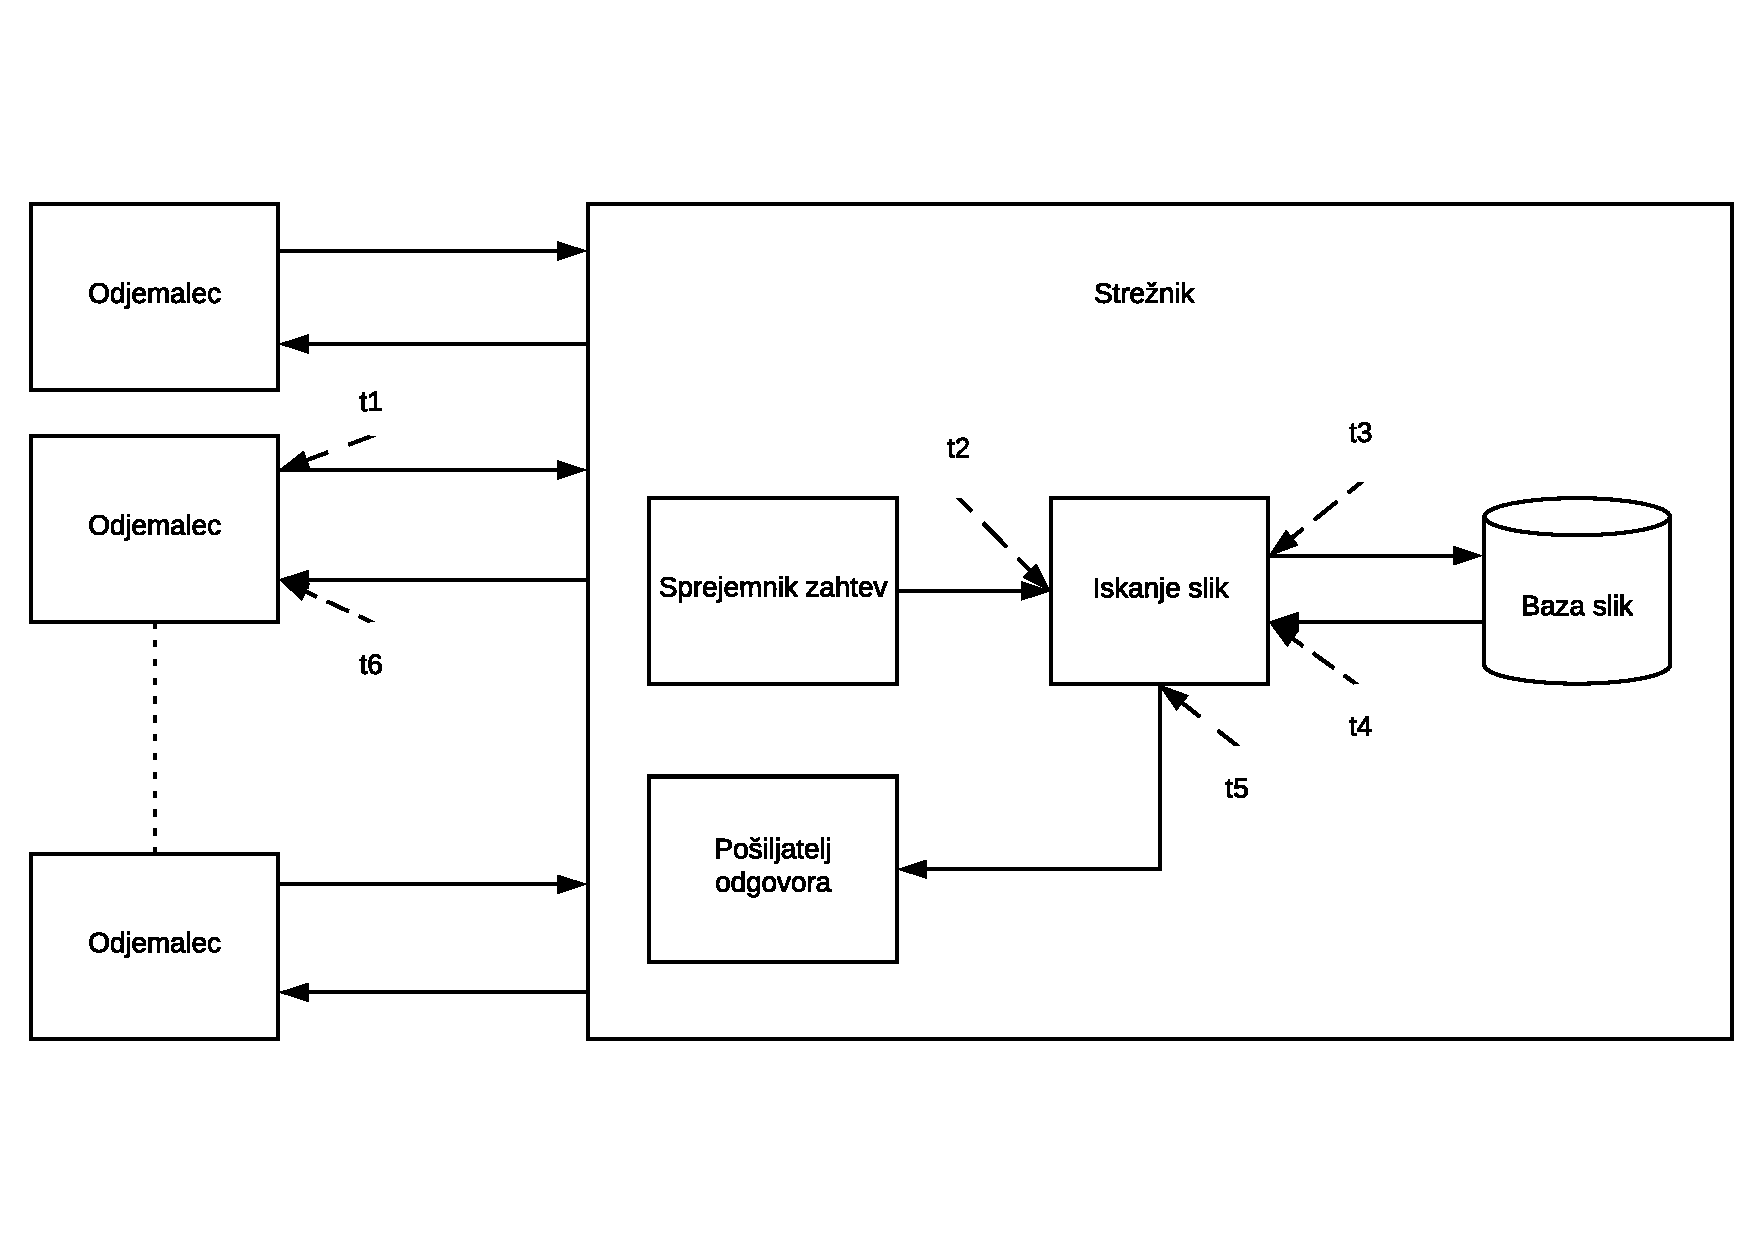
\includegraphics[scale=0.4]{Img/1_shema.pdf}
\caption{Shema opazovane storitve.}
\label{fig:1_osnovnaShema}
\end{figure}

\subsection{Tipi zahtev}

V osnovi vsi tipi zahtev vključujejo iskanje vzorca v naboru slik.
Razlikujejo se v tipu vzorca, ki ga uporabnik želi najti v sliki.
Storitev nudi tri tipe iskanj:
\begin{itemize}
\item iskanje specifične barve piksla,
\item iskanje piksla, podobnega specifični barvi,
\item iskanje slikovnega izseka.
\end{itemize}

\subsubsection{Iskanje specifične barve piksla}

Storitev prejme podatek o iskani barvi piksla.
Zaporedoma preiskuje slike v oblačni podatkovni bazi.
Takoj ko najde prvo pojavitev iskanega piksla, iskanje ustavi in vrne podatek o tej pojavitvi - zaporedna številka slike in koordinati $x$ ter $y$ najdenega piksla.
Če ne najde nobene pojavitve, preišče vse slike v podatkovni bazi in vrne sporočilo, da piksel ni bil najden.

\subsubsection{Iskanje piksla, podobnega specifični barvi}

Poleg iskane barve storitev prejme od odjemalca še največje dovoljeno odstopanje.
Zaporedoma preiskuje slike v podatkovni bazi, dokler ne najde prvega piksla, katerega barva se od iskane po komponentah razlikuje za največ toliko, kot določa odstopanje.
Razlika se izračuna po enačbi
\begin{multline} \label{1_eq_odstopanje}
Razlika(RGB_{piksel}, RGB_{iskan}) = \\ = |R_{piksel} - R_{iskan}| + |G_{piksel} - G_{iskan}| + |B_{piksel} - B_{iskan}|.
\end{multline}

Če je iskana barva naključno izbrana, potem lahko za dano odstopanje izračunamo približno verjetnost, da bomo dobili ujemanje z naključnim pikslom.
Za vsako barvo in odstopanje $n$ obstanja največ $\frac{1}{3}(n^3 + 6n^2 + 14n + 3)$ barv, ki se od iskane barve po komponentah razlikujejo za $n$.
Vsak barvni kanal lahko zavzema vrednosti od 0 do 255, torej je za izbiro barve na voljo $2^{24} = 16777216$ vrednosti.
Verjetnost aproksimiramo kot $\frac{n^3 + 6n^2 + 14n + 3}{3 \cdot 16777216}$.
Nekaj verjetnosti zadetka in ustreznih odstopanj: \\ % fix za preveč nabito postavitev

\begin{tabular}{c|c c c c c c c c}
verjetnost & 0.05\% & 0.1\% & 0.2\% & 0.5\% & 1\% & 2\% & 5\% & 10\% \\
\hline
odstopanje & 18 & 23 & 29 & 39 & 50 & 63 & 85 & 107
\end{tabular}
\\

Ampak piksli v slikah niso naključni.
Boljšo oceno dobimo, če privzamemo, da je barva cele slike \emph{približno} enaka - če ne najdemo ustreznega piksla na začetku slike, potem je velika verjetnost, da ga tudi v preostanku slike ne bomo.
Tako lahko izračunamo, koliko slik bo v povprečju pregledanih s pomočjo matematičnega upanja po formuli

\begin{equation} \label{1_eq_upanje}
E(p) = \sum_{i = 1}^{\text{število slik}} i \cdot (1 - p)^{i - 1} \cdot p = \frac{1}{p} .
\end{equation}

To pomeni, da bomo pri verjetnost 1\% v povprečju pregledali približno 100 slik pri vsaki zahtevi.
Izkaže se, da je ta ocena kar dobra v primeru te storitve.

\subsubsection{Iskanje slikovnega izseka}

Storitev prejme slikovni izsek.
Zaporedoma preiskuje slike v podatkovni bazi, dokler ne najde prvega ujemanja podanega izseka z izsekom na neki sliki.
Izseka se ujemata, če je barva vsakega piksla danega izseka za največ 7 oddaljena od barve ustreznega piksla na sliki.
Razlika barv se računa tako kot pri podobni barvi piksla (enačba \ref{1_eq_odstopanje}).
Odstopanje je tu potrebno le zato, ker pri shranjevanju izsekov pride do artifaktov stiskanja~\cite{1_wiki_compression}.

\subsection{Slikovni material}

Za potrebe zgoraj naštetih metod in njihovega testiranja smo na strežnik naložili 540 slik v JPEG formatu, ki smo jim zmanjšali velikost na 300 slikovnih pik po širini in 400 slikovnih pik po dolžini ali obratno za hitrejše procesiranje.
Hkrati nam to zagotavlja, da je časovna zahtevnost primerjave približno enaka za ves slikovni material.
Prav tako je bil cilj zbrati slike s čim večjo vsebinsko raznolikostjo, saj je to pomembno pri iskanju barve piksla in iskanju piksla podobnega specifični barvi.
Nekaj primerov slik se nahaja na sliki \ref{fig:1_sample_images}.

\begin{figure}[H]
    \centering
    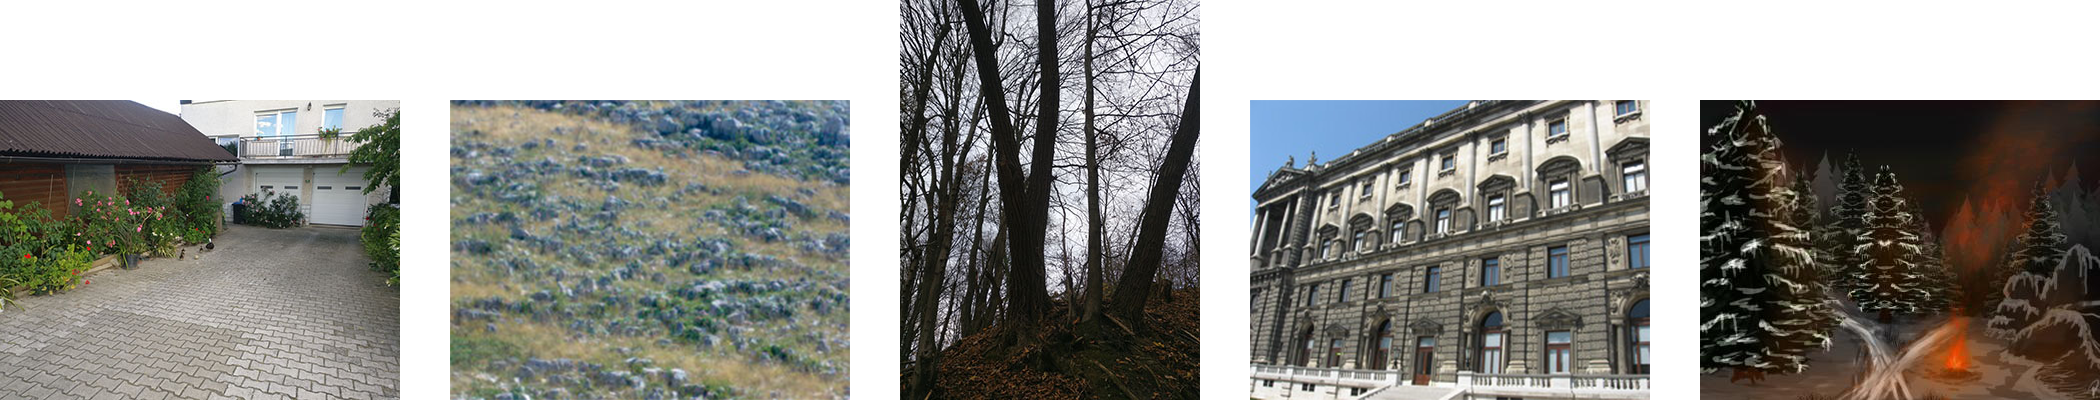
\includegraphics[scale=0.16]{Img/1_sample_images.png}
    \caption{Nekaj primerov slik iz nabora.}
    \label{fig:1_sample_images}
\end{figure}

\subsection{Amazon Web Services (AWS)}

Za delo z Amazon Web Services~\cite{1_aws_amazon} si moramo ustvariti račun v njihovem sistemu. Po uspešni registraciji si lahko ustvarimo svojo instanco EC2 storitve, ki nam jo Amazon ponuja zastonj za eno leto, pri čemer lahko na mesec porabimo največ 750 ur delovanja ponujenih instanc. Obsežnejša navodila so na voljo tudi na Amazonovi spletni strani~\cite{1_aws_amazon_tutorial}, mi pa to naredimo tako, da se postavimo v AWS Management Console~\cite{1_aws_amazon_console}, kjer lahko izberemo opcijo \emph{Launch a virtual machine with EC2}. Takoj nam konzola ponudi izbiro \emph{slike navideznega diska} - vnaprej priravljenega nabora datotek, ki ga lahko neposredno zaženemo na instanci~\cite{1_aws_amazon_ami}. Izbor možnih slik diska je prikazan na sliki \ref{fig:1_AWS_images}. Za naš projekt izberemo sliko Amazon Linux 2 AMI c.

\begin{figure}[H]
    \centering
    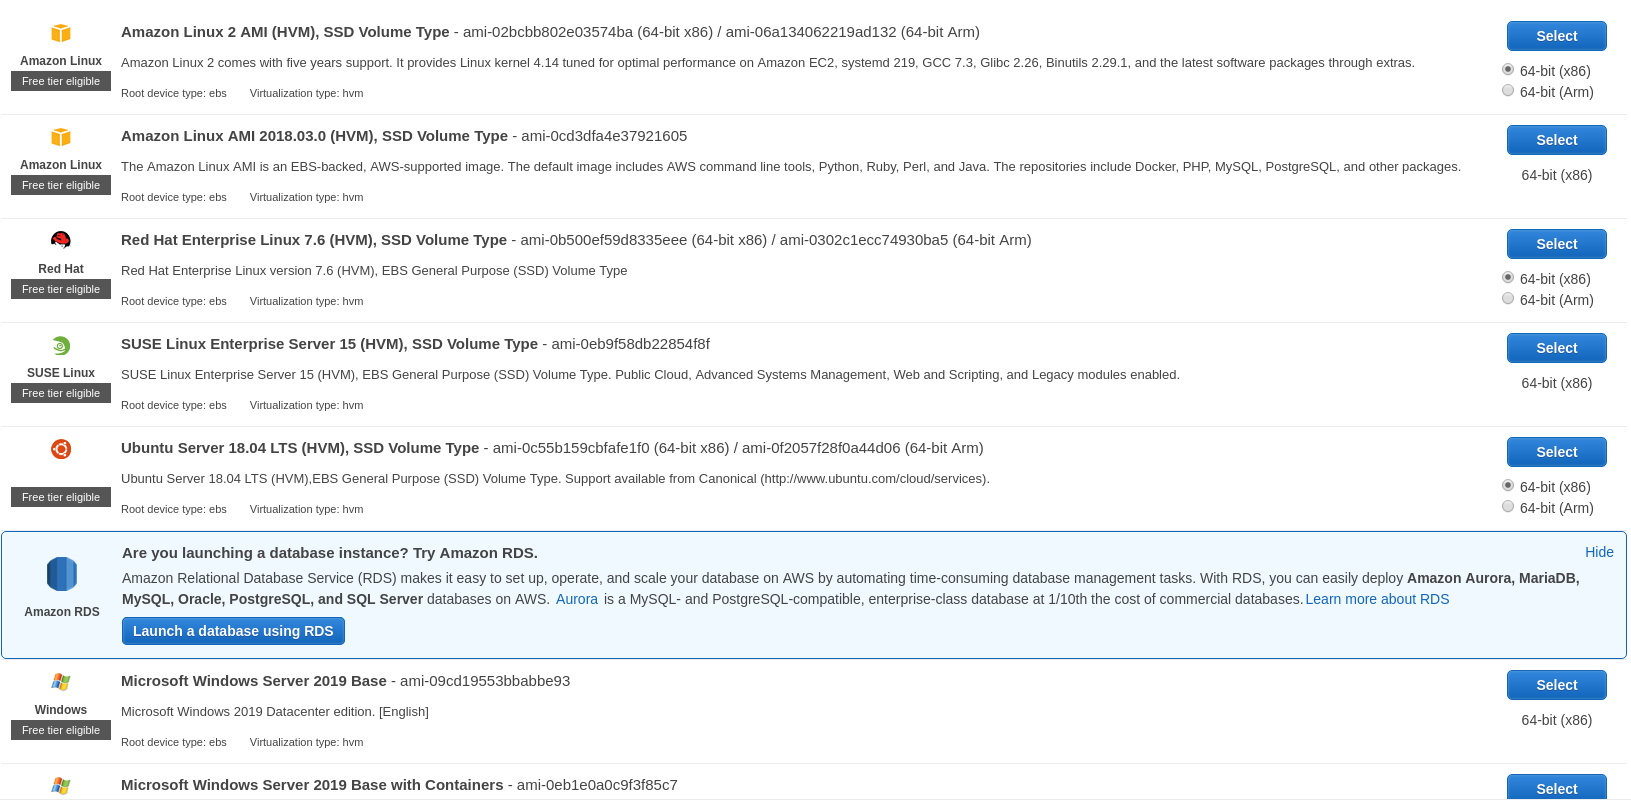
\includegraphics[scale=0.25]{Img/1_AWS_images.png}
    \caption{Slike navideznih diskov za izdelavo virtualke.}
    \label{fig:1_AWS_images}
\end{figure}

V naslednjem koraku izberemo tip instance slike, to je Amazonov način izbire paketov, ki vključujejo različne funkcionalnosti. Ker v našem primeru izbiramo brezplačno različico, nam ponujajo tip t2.micro, ki vsebuje 1 jedro, 1GB pomnilnika, nizko prioriteto hitrosti povezave do same instance strežnika (umetno omejena hitrost s spremenljivo največjo hitrostjo) in hrambo podatkov na platformi Elastic Block Storage, ki nam ponuja zastonjsko hranjenje podatkov na mrežno povezani shrambi~\cite{1_aws_amazon_ebs}. Za tem lahko nadaljujemo z nastavljanjem različnih konfiguracij naše virtualke ali pa preprosto kliknemo Review and Launch, ki nam ponudi še en pregled izbranih nastavitev in zažene virtualko. Po zagonu virtualke nam sistem ponudi opcijo generiranja para ključev za varno SSH povezavo do nje. Ko zaključimo z ustvarjanjem, se premaknemo v EC2 management console kjer kliknemo na \emph{instances}. Od tam lahko opazujemo status naše storitve in pridobimo tudi naslov, na katerem se nahaja. Za povezavo uporabimo javni naslov storitve, uporabnika $ec2-user$, za varnost pa uporabimo $.pem$ datoteko (Privacy Enhanced Mail Security Certificate), ki smo jo v prejšnjem koraku prenesli. Ko se uspešno povežemo na storitev, lahko pričnemo z razvojem naše aplikacije.

\subsection{Aplikacija}

Aplikacija je napisana v programskem jeziku Java, ki je interpretirana preko sprotnega prevajalnika, kar se lahko potencialno izkaže kot ozko grlo. Sestavljata jo odjemalska in strežniška komponenta, ki uporabljata skupne enumeratorje za določanje tipa zahteve. Zahteve sestavlja odjemalec in jih pošlja strežniku, ki te zahteve obdela - začne iskanje v slikah in pripravi prvi najden rezultat. Povezava med strežnikom in odjemalcem je trajna, dokler je eden od njiju ne prekine, kar nam omogoči, da pri meritvah ne upoštevamo časa vzpostavitve povezave. Podatki se prenašajo v obliki JSON, ki vsebuje sekvenčno številko zahteve, tip zahteve in morebitne dodatne podatke, ki so potrebni za obdelavo. V izpisu \ref{lst:JSON_req} je predstavljen primer zahteve v obliki dokumenta JSON, ki jo odjemalec pošlje strežniku.

\begin{lstlisting}[caption={Primer JSON zahteve.},label={lst:JSON_req}]
{
	"reqId": 1,
	"reqType": "PIXEL_NEAR",
	"pixelValue": "0xFFFA3881",
	"maxDistance": 86,
	"image": "",
	"req_start": 1555162220550,
	"err": ""
}
\end{lstlisting}

Strežnik ob prejemu podatkov začne z delom na ustrezni zahtevi ter nato pošlje odgovor klientu s številko zahteve in rezultatom. Odgovor vsebuje tudi čas proceiranja in branja slik. Strežniški del je napisan tako, da lahko paralelno obdeluje več zahtev. V izpisu  \ref{lst:JSON_res} je predstavljen primer odgovora na zahtevo, ki ga strežnik vrne odjemalcu.

\begin{lstlisting}[caption={Primer JSON odgovora.},label={lst:JSON_res}]
{
	"reqId": 1,
	"imageId": 4,
	"location": {
		"x": 124,
		"y": 87	
	},
	"proc_time": 4528,
	"req_start": 1555162220550,
	"image_fetch_time": 78,
	"err": ""
}
\end{lstlisting}

\section{Uporabljene metrike}

Kot glavno metriko bomo opazovali skupni čas zahteve in odgovora.

Podrobneje ga bomo razdelili na čas dostopa do datotečnega sistema (zbirke slik v mapi na datotečnem sistemu, recimo ji baza slik) ($t_{baza} = t_4 - t_3$) in celoten čas obdelave na strežniku ($t_{streznik} = t_5 - t_2$). Hkrati merimo celoten čas trajanja zahteve ($t_{zahteva} = t_6 - t_1$) (časi označeni na sliki \ref{fig:1_osnovnaShema}). Z izmerjenimi časi lahko izračunamo tudi druge kot sta čas procesiranja na strežniku ($t_{procesiranje} = t_{streznik} - t_{baza}$) in čas paketa na mreži ($t_{mreza} = t_{zahteva} - t_{streznik}$). S tem smo se znebili problema sinhronizacije ur med odjemalcem in strežnikom. Če bi želeli meriti tudi čas potovanja paketa od odjemalca na strežni in čas potovanja paketa od strežnika na odjemalec, pa bi potrebovali tudi sinhronizacijo ur, ker pa naš cilj ni meriti čase potovanja paketov, saj je to namreč lastnost omrežja in ne same platforme, bomo zadovoljni s skupnim časom paketa na mreži.

Zanima nas, kako se storitev odziva na zahteve ob različnih urah. Za potrebe meritev bomo odziv sistema merili ob treh različih časih v dnevu. Želimo izvedeti tudi, kako se časi odgovorov podaljšajo glede na število hkratnih uporabnikov.

\section{Meritve}

Zmogljivost storitve smo merili večkrat.
Testirali smo hitrost iskanja podobne barve, opazovali smo razlike v hitrosti odziva iz različnih lokacij in ob različnih časih.

\subsection{Poskusno testiranje}

V soboto, 27. aprila 2019 ob 20.37 smo poskusno testirali iskanje piksla v okolici barve.
Strežniku je bilo zaporedno poslanih 500 zahtev, vsaka je vsebovala naključno izbrano barvo, strežnik pa je iskal piksel z odstopanjem, manjšim ali enakim 50.
Odstopanje je bilo izbrano tako, da so bili zadetki čim bolj enakomerno razporejeni po slikah v podatkovni bazi.

Zahteve je generiral osebni računalnik, nahajajoč se na Viču v Ljubljani.
Prek brezžičnega omrežja je bil priklopljen na kabelski internet ponudnika A1, ki za zakupljen paket \emph{A1 Kombo L} oglašuje hitrost povezave 40 megabitov na sekundo k uporabniku in 10 megabitov na sekundo od uporabnika.
Test na strani \emph{Speedtest by Ookla} te vrednosti potrdi (rezultat testa: \url{https://www.speedtest.net/result/8218379266}).
Čas obhoda paketa od odjemalca do storitve in nazaj je povprečju znašal 62 milisekund.
Rezultat orodja \texttt{tracert} se nahaja v izpisu \ref{1_lst_tracert}.

\begin{lstlisting}[caption={Rezultat orodja \texttt{tracert}.},label={1_lst_tracert}]
Tracing route to ec2-52-212-203-50.eu-west-1.compute.amazonaws.com [52.212.203.50]
over a maximum of 30 hops:

  1     2 ms    <1 ms    <1 ms  192.168.1.254
  2     *        *        *     Request timed out.
  3     *        *        *     Request timed out.
  4     *        *        *     Request timed out.
  5    25 ms    26 ms    25 ms  195.3.102.57
  6     *        *        *     Request timed out.
  7    26 ms    26 ms    28 ms  lg4-9072.as8447.a1.net [195.3.64.142]
  8    26 ms    27 ms    25 ms  52.95.219.250
  9    31 ms    33 ms    32 ms  52.93.38.102
 10    25 ms    26 ms    27 ms  52.93.38.109
 11     *       58 ms    57 ms  54.239.44.47
 12    63 ms    58 ms    58 ms  52.93.128.141
 13    57 ms    60 ms    58 ms  52.93.128.2
 14     *       58 ms    63 ms  54.239.44.158
 15     *        *        *     Request timed out.
 16    72 ms    93 ms    80 ms  52.93.7.190
 17    59 ms    62 ms    59 ms  52.93.101.127
 18    72 ms     *       79 ms  52.93.101.126
 19    61 ms    61 ms    61 ms  52.93.36.143
 20     *        *        *     Request timed out.
 21     *        *        *     Request timed out.
 22     *        *        *     Request timed out.
 23     *        *        *     Request timed out.
 24     *        *        *     Request timed out.
 25     *        *        *     Request timed out.
 26     *        *        *     Request timed out.
 27    60 ms    62 ms    60 ms  ec2-52-212-203-50.eu-west-1.compute.amazonaws.com [52.212.203.50]

Trace complete.
\end{lstlisting}

Celotni časi zahtev ($t_{zahteva}$) so prikazani na sliki \ref{fig:1_poskusno_total_times_unordered}.

\begin{figure}[H]
	\centering
	\scriptsize
	\begin{tikzpicture}[scale=1.1]
		\begin{axis}[xlabel={Zaporedna številka zahteve}, xtick={0,100,...,500}, minor xtick={0,20,...,500}, ylabel={$t_{zahteva}$ [ms]}, ytick={0,1000,...,7000}, minor ytick={0,200,...,7000}, grid=major]
			\addplot[mark=none] table{Result_processing/27_04_poskusno/1_test_total_times_unordered.dat};
		\end{axis}
	\end{tikzpicture}
	\caption{Diagram celotnih časov zahtev.}
	\label{fig:1_poskusno_total_times_unordered}
\end{figure}

Najhitrejši odziv je znašal 63 milisekunde, najdaljši pa 6778 milisekund.
V povprečju je čas odziva znašal 587 milisekund.

Iz slike \ref{fig:1_poskusno_total_times_unordered} ni enostavno razvidno, kakšna je razporeditev časov zahtev.
Na sliki \ref{fig:1_poskusno_total_times} so celotni časi zahtev ($t_{zahteva}$) prikazani po velikosti urejeni.

\begin{figure}[H]
	\centering
	\scriptsize
	\begin{tikzpicture}[scale=1.1]
		\begin{axis}[xlabel={Število zahtev}, xtick={0,100,...,500}, minor xtick={0,20,...,500}, ylabel={$t_{zahteva}$ [ms, naraščajoče]}, ytick={0,1000,...,7000}, minor ytick={0,200,...,7000}, grid=major]
			\addplot[mark=none] table{Result_processing/27_04_poskusno/1_test_total_times.dat};
		\end{axis}
	\end{tikzpicture}
	\caption{Diagram celotnih časov zahtev, urejenih naraščajoče po velikosti.}
	\label{fig:1_poskusno_total_times}
\end{figure}

Iz slike \ref{fig:1_poskusno_total_times} je lažje razvidno, da je večina časov zahtev manj kot 500 milisekund, le peščica jih preseže 3500 milisekund.

Časi paketa na mreži ($t_{mreza}$) so po velikosti urejeni prikazani na sliki \ref{fig:1_poskusno_transfer_times}.
Najhitrejši čas obhoda je znašal 60 milisekund, najdaljši pa 395 milisekund.
V povprečju je čas paketa na mreži znašal 64 milisekund, v 499 izmed 500 primerov ni presegel 78 milisekund.

\begin{figure}[H]
	\centering
	\scriptsize
	\begin{tikzpicture}[scale=1.1]
		\begin{axis}[xlabel={Število zahtev}, xtick={0,100,...,500}, minor xtick={0,20,...,500}, ylabel={$t_{mreza}$ [ms, naraščajoče]}, ytick={0,100,...,400}, minor ytick={0,10,...,400}, grid=major]
			\addplot[mark=none] table{Result_processing/27_04_poskusno/1_test_transfer_times.dat};
		\end{axis}
	\end{tikzpicture}
	\caption{Diagram časov obhoda paketa, urejenih naraščajoče po velikosti.}
	\label{fig:1_poskusno_transfer_times}
\end{figure}

V splošnem nas zanima, koliko časa vzame nalaganje slik z diska v pomnilnik ($t_{baza}$), kolikšen del procesiranja zavzame nalaganje slik ($\frac{t_{baza}}{t_{streznik}}$) in koliko časa v povprečju zavzame nalaganje ene slike v pomnilnik ($\frac{t_{baza}}{N_{nalozenih}}$).

Časi, ki jih storitev porabi za nalaganje slik v pomnilnik, so po velikosti urejeni prikazani na sliki \ref{fig:1_poskusno_loading_time_absolute}.
Zavzemajo vrednosti med 1 in 4008 milisekund, v povprečju pa 201 milisekundo.

\begin{figure}[H]
	\centering
	\scriptsize
	\begin{tikzpicture}[scale=1.1]
		\begin{axis}[xlabel={Število zahtev}, xtick={0,100,...,500}, minor xtick={0,20,...,500}, ylabel={$t_{baza}$ [ms, naraščajoče]}, ytick={0,1000,...,4000}, minor ytick={0,200,...,4000}, grid=major]
			\addplot[mark=none] table{Result_processing/27_04_poskusno/1_test_loading_time_absolute.dat};
		\end{axis}
	\end{tikzpicture}
	\caption{Diagram časov, porabljenih za nalaganje slik z diska v pomnilnik, urejenih naraščajoče po velikosti.}
	\label{fig:1_poskusno_loading_time_absolute}
\end{figure}

Odstotki časa, ki ga storitev porabi za nalaganje slik v pomnilnik, so po velikosti urejeni prikazani na sliki \ref{fig:1_poskusno_loading_time_percentage}.
Zavzemajo vrednosti med 16 in 100 odstotkov, v povprečju pa 36 odstotkov.

\begin{figure}[H]
\centering
\scriptsize
	\begin{tikzpicture}[scale=1.1]
		\begin{axis}[xlabel={Število zahtev}, xtick={0,100,...,500}, minor xtick={0,20,...,500}, ylabel={$\frac{t_{baza}}{t_{streznik}}$ [odstotek, naraščajoče]}, ytick={0,20,...,100}, minor ytick={0,2,...,100}, grid=major]
			\addplot[mark=none] table{Result_processing/27_04_poskusno/1_test_loading_time_percentage.dat};
		\end{axis}
	\end{tikzpicture}
\caption{Diagram odstotkov časa, porabljenega za nalaganje slik z diska v pomnilnik, urejenih naraščajoče po velikosti.}
\label{fig:1_poskusno_loading_time_percentage}
\end{figure}

Povprečne vrednosti časa nalaganja 1 slike so prikazani na sliki \ref{fig:1_poskusno_pic_loading_time}.
Vrednosti so izračunane kot količnik časa nalaganja slik s številom preiskanih slik pri posamezni zahtevi.
Zavzemajo vrednosti med 1 in 200 milisekund, v povprečju 4 milisekunde.
V 493 izmed 500 primerov ni presegel 7 milisekund.

\begin{figure}[H]
\centering
\scriptsize
	\begin{tikzpicture}[scale=1.1]
		\begin{axis}[xlabel={Zaporedna številka zahteve}, xtick={0,100,...,500}, minor xtick={0,20,...,500}, ylabel={Čas nalaganja 1 slike [ms]}, ytick={0,50,...,200}, minor ytick={0,10,...,200}, grid=major]
			\addplot[mark=none] table{Result_processing/27_04_poskusno/1_test_pic_loading_time.dat};
		\end{axis}
	\end{tikzpicture}
\caption{Diagram povprečnih časov nalaganja ene slike z diska v pomnilnik, v vrstnem redu zahtev.}
\label{fig:1_poskusno_pic_loading_time}
\end{figure}

\subsection{Primerjava odzivov na zahteve iz različnih lokacij}

Zaradi odločitve, da bomo testirali tudi z različnih lokacij, smo se najprej odločili, da preverimo kakšne zakasnitve (ping) ima posamezen član na različnih lokacijah do strežnika. Rezultati po 30 ponovitvah so prikazani v tabeli \ref{1_tab_ping}. Te razlike v časih pripisujemo predvsem temu dejstvu, da ima vsaka od teh lokacij drugega ponudnika omrežnih storitev in zato naši paketi prepotujejo različne poti in opravijo v povprečju 7 skokov, dokler ne pridejo do skupne točke, ki pa je že v lasti podjetja Amazon Technologies Inc.~\cite{1_ip_location}. Te razlike so pomembne samo pri merjenju časa, ko se paket nahaja na mreži, in niso odvisne od zmogljivosti same storitve.

\begin{table}[ht]
 \caption{Rezultat orodja \texttt{ping}}
 \label{1_tab_ping}
 \centering
\begin{tabular}{ |p{3cm}||p{2cm}|p{2cm}|p{2cm}| }
 \hline
 Lokacija&Min [ms]&Max [ms]&Povprečje[ms]\\
 \hline
 Ljubljana Vič   & 58    &62&   58\\
 Postojna &   41  & 41   &41\\
 Vrtojba &42 & 43&  42\\
 \hline
\end{tabular}
\end{table}

\subsection{Primerjava odzivov na zahteve ob različnih časih}

Kvaliteta storitve je odvisna tudi od zmožnosti odzivanja ob različnih časih.
To smo testirali tako, da smo v urnih intervalih pošiljali zaporedno 500 zahtev tipa iskanja piksla, podobnega specifični barvi.
Vsaka zahteva je vsebovala naključno izbrano barvo, strežnik pa je iskal piksel z odstopanjem, manjšim ali enakim 50.
Povprečni časi glede na uro so prikazani na sliki \ref{fig:1_hourly_response_time_averages}.

\begin{figure}[H]
\centering
\scriptsize
	\begin{tikzpicture}[scale=1.1]
		\begin{axis}[xlabel={Ura}, xtick={0,3,...,24}, ymin = 0, ymax = 1000, ylabel={Povprečen čas odgovora [ms]}, ytick={0,100,...,1000}, minor ytick={0,20,...,1000}, grid=major]
			\addplot[mark=none] table{Result_processing/02_05_razlicne_ure/avgs.dat};
		\end{axis}
	\end{tikzpicture}
\caption{Diagram povprečnih časov odziva glede na čas v dnevu.}
\label{fig:1_hourly_response_time_averages}
\end{figure}

V grobem se storitev odziva približno enako skozi dan, dopoldan in zgodaj zvečer nekoliko hitreje kot pozno popoldan in pozno zvečer.

\section{Plan dela}

\begin{itemize}
\item testiranje ostalih dveh iskanj
\item testiranje iz različnih lokacij
\item testiranje ob različnih časih
\item iskanje barve z odstopanjem: testiranje razlik med odstopanji
\item testiranje z več sočasnimi uporabniki
\item določitev orodij - avtomatizacija merjenja, zbiranje rezultatov
\item premislek o skalabilnosti
\end{itemize}

\inputencoding{cp1250}
